\chapter{METHODOLOGY}
\section{Iterative Approach}
Iterative development is a methodology where a project is broken down into smaller, manageable parts or iterations, each delivering a piece of functionality that is tested and refined before moving on to the next iteration. Here are the steps for iterative development, particularly applicable to developing a fake news detection system like TrueLens:
\begin{itemize}
    \setlength\itemsep{0.25em}
    \item Planning and Requirements Gathering
    \item Planning and Design
    \item Development and Implementation
    \item Testing and Quality Assurance
    \item Review and Evaluation
    \item Deployment and Release
    \item Feedback and iteration
    \item Documentation and Maintenance
\end{itemize}
\section{Requirement Analysis}
\section{Feasibility Analysis}
Feasibility analysis is a systematic assessment of the practicality, viability, and potential success of a proposed project or initiative. It evaluates various aspects including technical, operational, economic, legal, and schedule feasibility to determine whether the project can be realistically implemented and achieve its intended objectives. Feasibility analysis helps stakeholders make informed decisions by identifying risks, constraints, and opportunities associated with the project, ultimately guiding resource allocation and planning to maximize the likelihood of successful outcomes.
\subsection{Financial Feasibility}
For the TrueLens project, our toolkit includes Django for robust backend development, Python for scripting and backend logic, PostgreSQL for efficient database management, and a combination of HTML, CSS, and JavaScript for dynamic frontend implementation. Additionally, Figma will be used for designing user interfaces. Our main financial allocation will be dedicated to securing reliable server hosting to ensure optimal performance and seamless accessibility of the system.
\subsection{Operational Feasibility}
Operational feasibility for the TrueLens project involves assessing user acceptance among stakeholders like media consumers, journalists, and fact-checkers. It includes providing adequate training and support, ensuring compliance with data protection regulations and ethical standards, and evaluating scalability to meet growing demands effectively. These factors ensure the system is practical, user-friendly, and capable of maintaining trust while combating misinformation.  
\subsection{Technical Feasibility}
Technical feasibility for the TrueLens project involves evaluating several critical factors to ensure its successful implementation. This includes assessing the availability of expertise in machine learning (ML) algorithms and frameworks such as PyTorch or TensorFlow, essential for developing accurate fake news detection models. Integration with Django for backend development must be evaluated to ensure seamless compatibility and optimal performance, especially concerning scalability requirements to handle large datasets and real-time processing effectively. Additionally, robust infrastructure planning is necessary to support the system's technological needs and future growth.
\newpage
\section{System Design}
\subsection{Architecture Design}
The following diagram shows diagram of our Architecture. Mainly shows what are the functions can be accessed after starting our application.
\begin{figure}[H]
    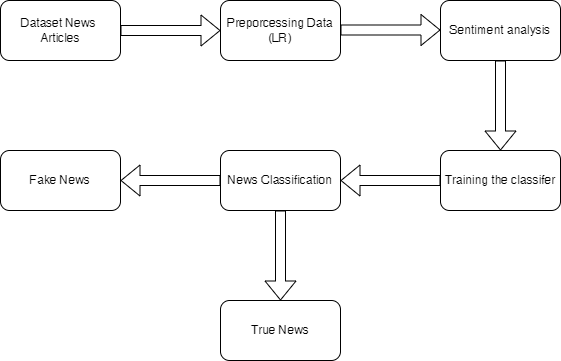
\includegraphics[height = 8cm]{Diagrams/New system.drawio.png}
    \caption{Main Architecture of System}
\end{figure}
\newpage
\subsection{Data Modelling(ER-Diagram)}
ER Diagram is mainly used to design database schema. With the help of below er diagram we can easily design database in SQL.
\begin{figure}[H]
    \rotatebox{90}{
    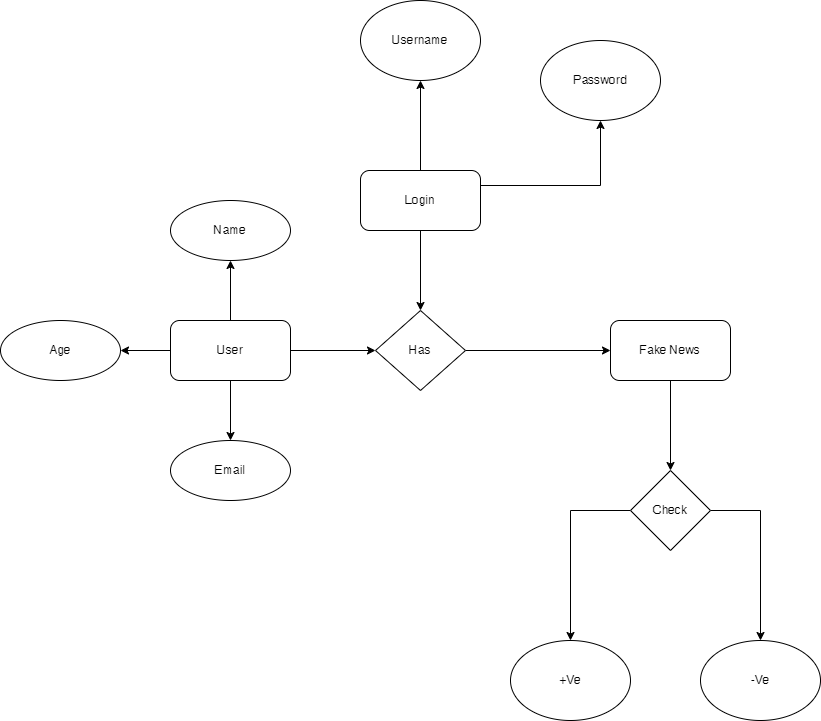
\includegraphics[height = 12cm]{Diagrams/ER new.drawio.png}}
    \caption{ER Diagram of System Data}
\end{figure}
\newpage
\subsection{Activity Diagram}
An activity diagram visually presents a series of actions or flow of control in a system similar to a flowchart or a data flow diagram. This diagram showed how our program flow goes on.
\begin{figure}[H]
   \centering
    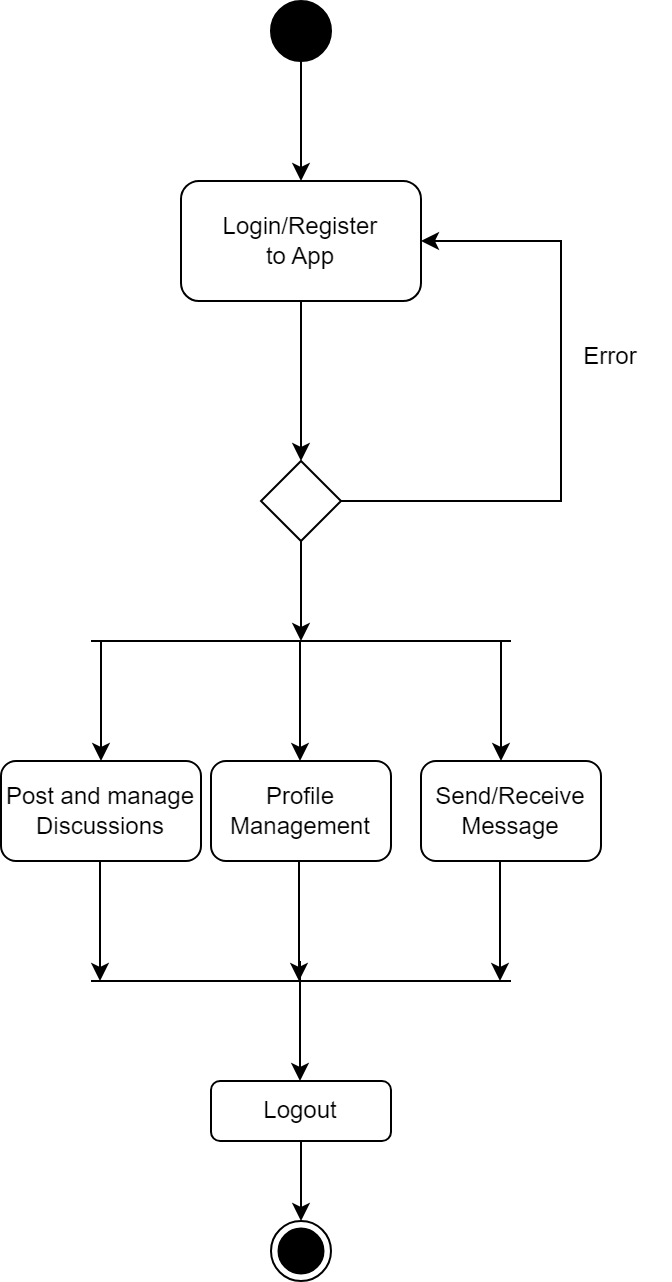
\includegraphics[height = 15cm]{Diagrams/Activity.drawio.png}
    \caption{Activity Diagram}
\end{figure}
\newpage
\subsection{DFD}
DFD or Data Flow Diagram is mainly used to show how data are being flowed in and out of our system. There are 3 levels of DFD i.e Context Level(Level 0),Level 1 and Level 2
\begin{figure}[H]
    \centering
    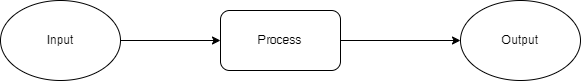
\includegraphics[height = 2cm]{Diagrams/dfd0new.drawio.png}
    \caption{Data Flow Diagram (Context Level)}
\end{figure}
\newpage
\subsection{Use Case Diagram}
A use case diagram, part of UML, visually represents interactions between actors and a system. Actors are external entities, while use cases depict specific functionalities. Relationships, such as association, generalization, include, and extend, illustrate connections between actors and use cases. The diagram helps in understanding system behavior, requirements, and scope.
\begin{figure}[H]
    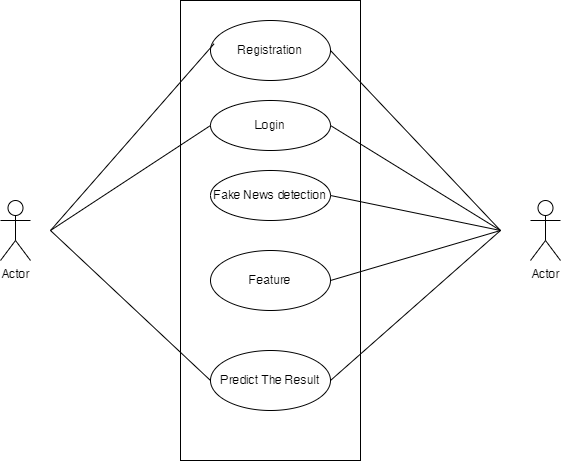
\includegraphics[height = 10cm]{Diagrams/Use-case.drawio.png}
    \caption{Use Case Diagram}
\end{figure}
